\documentclass[a4paper,12pt]{report}
\usepackage[italian]{babel}
\usepackage{amsmath,amssymb,amsthm}
\usepackage[top=5cm,bottom=5cm,left=4cm,right=4cm]{geometry}
\usepackage{graphicx,float}
\usepackage{caption,subcaption}
\usepackage{multirow}
\usepackage[shortlabels]{enumitem}
\usepackage{booktabs}
\usepackage[hidelinks]{hyperref}
\usepackage[style=numeric,sorting=nty,backend=bibtex]{biblatex}

\newtheorem{The}{Teorema}
\newtheorem{Tec}{Tecniche notevoli}
\newtheorem{Res}{Risultato}
\newtheorem{Lem}[Res]{Lemma}
\newtheorem*{Def}{Definizione}

\newcommand{\Chapter}[2]{\chapter[#1]{#1\\[1ex]\large#2}}

\includeonly
{
	chapters/integrale_gauss.tex,
 	chapters/funzione_gamma.tex,
 	chapters/costante_eulero_mascheroni.tex, 
 	chapters/approx_de_moivre_sterling.tex, 
	chapters/sophomore_dream.tex
}

\author{S. Licciardi\thanks{simone.licciardi@mail.polimi.it}, PoliMI undergraduate}
\date{\large Anno accademico 2023-2024}
\title
{
	\large Complementi di\\
	\LARGE \textbf{Analisi Matematica I} \\[.4\baselineskip]
	\large Appunti dalla lezione Turbo di V. Pata, Politecnico di Milano
}

\begin{document}
\maketitle
\tableofcontents

\par\vspace{2cm}Queste note nascono per ordinare gli appunti della Lezione Turbo del corso di Analisi Matematica 1 del professore V. Pata. 
Mentre il resto del corso è completato dagli appunti del docente, è nello spirito di questa lezione che non sia così.

Quindi, l'obiettivo non è soddisfare la curiosità dello studente "che si porta avanti", quanto permettergli di ricordarsi a distanza di tempo gli argomenti trattati.

Il docente è a conoscenza dell'esistenza di queste note, ma non sono nè ufficialmente nè ufficiosamente state approvate in alcuna maniera.

\newpage

% integrale_gauss.tex
%! TeX root = ../lezione_turbo.tex

\chapter{Integrale di Gauss}

\begin{Def}
	Per funzione gaussiana si intende l'applicazione
	\begin{equation*}
		f: x \in \mathbb{R} \to e^{-x^2} \in \mathbb{R}.
	\end{equation*}
\end{Def}

In questo capitolo la studiamo e forniamo un importante risultato preliminare: il valore del suo integrale improprio.
%Essa è di fondamentale importanza non solo nella statistica e nella probabilità, ma anche nell'analisi matematica, dove può essere impiegata per ricavare il valore di alcuni integrali che non ammettono una primitiva elementare.
%Essa è un esempio di funzione non \textit{elementare}: non è una funzione algebrica, esponenziale, logaritmica, nè se si ottiene da operazioni aritmetiche o dalla composizione.

Partiamo da alcune proprietà utili per trovarlo. La funzione è continua su $ \mathbb{R}$ ed è quindi localmente integrabile e ammette primitiva. 
Si può dimostrare che quest'ultima non è però \textit{elementare}, e cioè non può essere espressa attraverso operazioni tra e composizioni di funzioni algebriche, esponenziali o logaritmiche. 
Pertanto, anche se è teoricamente possibile calcolare l'integrale su un qualsiasi intervallo reale con il Teorema Fondamentale del Calcolo, non si dispone degli strumenti operativi per farlo. 
Per questo, il nostro obiettivo sarà determinare l'integrale improprio sull'intero dominio reale.

\begin{Res}[Integrale di Gauss]
	\label{res_1}
	\begin{equation*}
		\, \int_{- \infty}^{+ \infty}e^{-x^2} \, \mathrm{d}x = \sqrt{ \pi}
	\end{equation*}
\end{Res}
\begin{proof}[Dimostrazione - Integrabilità]
	Poichè l'intervallo su cui si calcola l'integrale non è limitato, si tratta di un integrale improprio. 
	Per continuità della funzione, i punti critici (in cui verificare l'integrabilità) sono i soli estremi dell'intervallo.

	Per parità, ci limitiamo a $ \left[ \,0,+ \infty \right)$, dove per $x \geq 1$ vale $e^{x^2} > x^2$, da cui segue che $x^{-2} \geq e^{-x^2}$. 
	Allora, per il criterio del confronto si ha che 
	\begin{equation*}
		\, \int_{1}^{+ \infty} x^{-2} \, \mathrm{d}x \geq \, \int_{1}^{+ \infty} e^{-x^2} \, \mathrm{d}x, 
	\end{equation*}
	e quindi $e^{-x^2} \in \mathbb{I} \,( \mathbb{R})$.
\end{proof}
\begin{proof}[Dimostrazione - Valore]
	Poniamo
	\begin{equation*}
		\mathrm{I} = 
		\, \int_{0}^{+ \infty}e^{-x^2} \, \mathrm{d}x,
	\end{equation*}
	e per parità dell'integranda
	\begin{equation*}
		\, \int_{- \infty}^{+ \infty}e^{-x^2} \, \mathrm{d}x = 
		2 \, \mathrm{I}.
	\end{equation*}
	Calcoliamo la quantità al quadrato. Per linearità, possiamo innestare gli integrali (che si comportano come delle costanti). 
	In particolare, vale la seguente uguaglianza.
	\begin{equation*}
		\mathrm{I}^2 = 
		\int_{0}^{+ \infty} \mathrm{I} \, \left(e^{-x^2} \right) \, \mathrm{d}x=
		\, \int_{0}^{+ \infty} \left( \, \int_{0}^{+ \infty} e^{-x^2} \, \mathrm{d}x \right) e^{-y^2} \, \mathrm{d}y
	\end{equation*}
	Per linearità, portiamo $e^{-y^2}$ nell'integrale interno ed effettuiamo il cambio di variabili $t = \frac{x}{y}$ (con l'identità formale $ \, \mathrm{d}x=y \, \mathrm{d}t$). Si ottiene
	\begin{equation*}
		\mathrm{I}^2 = 
		\, \int_{0}^{+ \infty} \left( \, \int_{0}^{+ \infty} ye^{-y^2(1+t^2)} \, \mathrm{d}t \right) \, \mathrm{d}y.
	\end{equation*}
	Per il Teorema di Fubini\footnote{Ri} (che, in questo caso, richiede la continuità dell'integranda), scambiamo le variabili di integrazione. 
	Calcoliamo la primitiva dell'integrale interno nella variabile $y$ (e cioè, considerando $t$ costante) e la valutiamo con il Teorema Fondamentale del Calcolo.
	\begin{equation*}
		\begin{split}
			\mathrm{I}^2 
			& =
			\, \int_{0}^{+ \infty} \left( \, \int_{0}^{+ \infty} ye^{-y^2(1+t^2)} \, \mathrm{d}y \right) \, \mathrm{d}t= 
			\\ &=
			- \frac{1}{2} \, \int_{0}^{+ \infty} \frac{1}{1+t^2} \ \left[ e^{-y^2(1+t^2)} \right]_{0}^{+ \infty} \, \mathrm{d}t= 
			\\ &= 
			\frac{1}{2} \, \int_{0}^{+ \infty} \frac{1}{1+t^2} \, \mathrm{d}t = \frac{ \pi}{4}
		\end{split}
	\end{equation*}
	Segue il risultato.
\end{proof}
\pagebreak

% funzione_gamma.tex
%! TeX root = ../lezione_turbo.tex
\Chapter{Funzione Gamma di Eulero}{"La più bella funzione dell'analisi matematica" \footnote{Come reference, si consiglia \textit{Emil Artin, The Gamma Function}}}

\begin{Def} 
Per funzione Gamma di Eulero si intende l'applicazione $ \Gamma:(0,+ \infty) \to \mathbb{R}$ data da
	\begin{equation*}
		\Gamma(x)= 
		\int_{0}^{+ \infty}e^{-t} \,t^{ \,x-1} \, \mathrm{d}t.
	\end{equation*}
\end{Def}
Osserviamo che la definizione è ben posta: l'integrabilità impropria dell'integranda è immediata sia in un intorno di $+ \infty$ che in uno di $0$ per ogni $t$ reale.

Iniziamo dalla derivabilità. 
Assumendo che certe ipotesi di regolarità siano soddisfatte, la catena di uguaglianze
\begin{equation*}
\begin{split}
	\Gamma'(x) 
	&= 
	\frac{ \partial}{ \partial x} \int_{0}^{+ \infty} e^{-t} \,t^{ \,x-1} \, \mathrm{d}t = 
	\int_{0}^{+ \infty} \frac{ \partial}{ \partial x} \left(e^{-t} \,t^{ \,x-1} \right) \, \mathrm{d}t = 
	\\ &= 
	\int_{0}^{+ \infty} e^{-t} \,t^{ \,x-1} \log t \, \mathrm{d}t
\end{split}
\end{equation*}
determina la prima derivata. 
Induttivamente, si ottiene che
\begin{equation*}
	\Gamma^{(n)}(x) = 
	\int_{0}^{+ \infty} e^{-t} \,t^{ \,x-1} \log^n t \, \mathrm{d}t,
\end{equation*}
dove l'integrabilità per ogni $n$ garantisce che $ \Gamma$ sia di classe $C^{ \infty}$. 
In particolare, la funzione è derivabile e per $x=1$ si ottiene un risultato degno di nota:
\begin{equation*}
	\Gamma'(1)= 
	\int_{0}^{+ \infty} \log t \, e^{-t} \, \mathrm{d}t = 
	- \gamma.
\end{equation*}
Riportiamo, senza dimostrazione, che la funzione è addirittura analitica. 

%%%%%%

Passiamo alla convessità. 
Nel seguito, utilizzeremo la disuguglianza di Young:
\begin{equation}
	\label{young_ineq}
	ab \leq \lambda a^ \frac{1}{ \lambda} + (1- \lambda) b^ \frac{1}{1- \lambda},	
\end{equation}
dove $a,b \in \mathbb{R}$ e $ \lambda \in \left(0,+ \infty \right)$. 

La si può dimostrare utilizzare la convessità dell'esponenziale e le sue proprietà:
\begin{equation*}
\begin{split}
	ab 
	& = 
	\exp \left( \log a + \log b \right) = 
	\exp \left({ \lambda \log a^ \frac{1}{ \lambda} + \left(1- \lambda \right) \log b^ \frac{1}{1- \lambda}} \right) \leq 
	\\ & \leq \lambda \exp \left( \log a^ \frac{1}{ \lambda} \right) + \left(1- \lambda \right) \exp \left( \log b^ \frac{1}{1- \lambda} \right) = 
	\lambda a^ \frac{1}{ \lambda} + \left(1- \lambda \right) b^ \frac{1}{1- \lambda}.
\end{split}
\end{equation*}
La convessità di $ \Gamma$, equivalente alla disuguglianza
\begin{equation*}
	\Gamma( \lambda a + (1- \lambda) b) \leq \lambda \Gamma(a) + (1- \lambda) \Gamma(b)
\end{equation*}
per ogni $a,b \in \left(0,+ \infty \right)$ e $ \lambda \in \left(0,+ \infty \right)$, segue dalla catena di relazioni
\begin{equation*}
\begin{split}
	\Gamma( \lambda a + (1- \lambda) b) 
	&= 
	\int_{0}^{+ \infty}e^{-t} \,t^{ \lambda a + (1- \lambda) b -1} \, \mathrm{d}t = 
	\\ &= 
	\int_{0}^{+ \infty}e^{-t} \,t^{ \lambda (a-1) + (1- \lambda) (b-1)} \, \mathrm{d}t \leq
	\\ &\leq 
	\int_{0}^{+ \infty}e^{-t} \left( \lambda t^{a-1} + (1- \lambda) t^{b-1} \right) \, \mathrm{d}t =
	\\ &=
	\lambda \Gamma(a) + (1- \lambda) \Gamma(b).
\end{split}
\end{equation*}
Ci sono poi alcuni punti in cui è facile computare il valore della funzione.
Nel punto $x=1$ abbiamo 
\begin{equation*}
	\Gamma(1)= 
	\int_{0}^{+ \infty}e^{-t} \, \mathrm{d}t= \left[ e^{-t} \right]_0^{+ \infty}=
	1.
\end{equation*}

Per $x=2$, invece, è sufficiente integrare per parti. Infatti, 
\begin{equation*}
	\Gamma(2) =
	\int_{0}^{+ \infty} te^{-t} \, \mathrm{d}t =
	\left[ - \frac{t}{e^t} \right]_0^{+ \infty} + \int_{0}^{+ \infty} e^{-t} \, \mathrm{d}t =
	\Gamma(1) =
	1.
\end{equation*}

Terminiamo la descrizione qualitativa della funzione con i limiti
\begin{equation*}
	\lim \limits_{x \to0^+} \Gamma(x) =
	+ \infty \qquad \lim \limits_{x \to+ \infty} \Gamma(x) =
	+ \infty,
\end{equation*}
e ricaviamo che il grafico
\begin{figure}
	\centering
	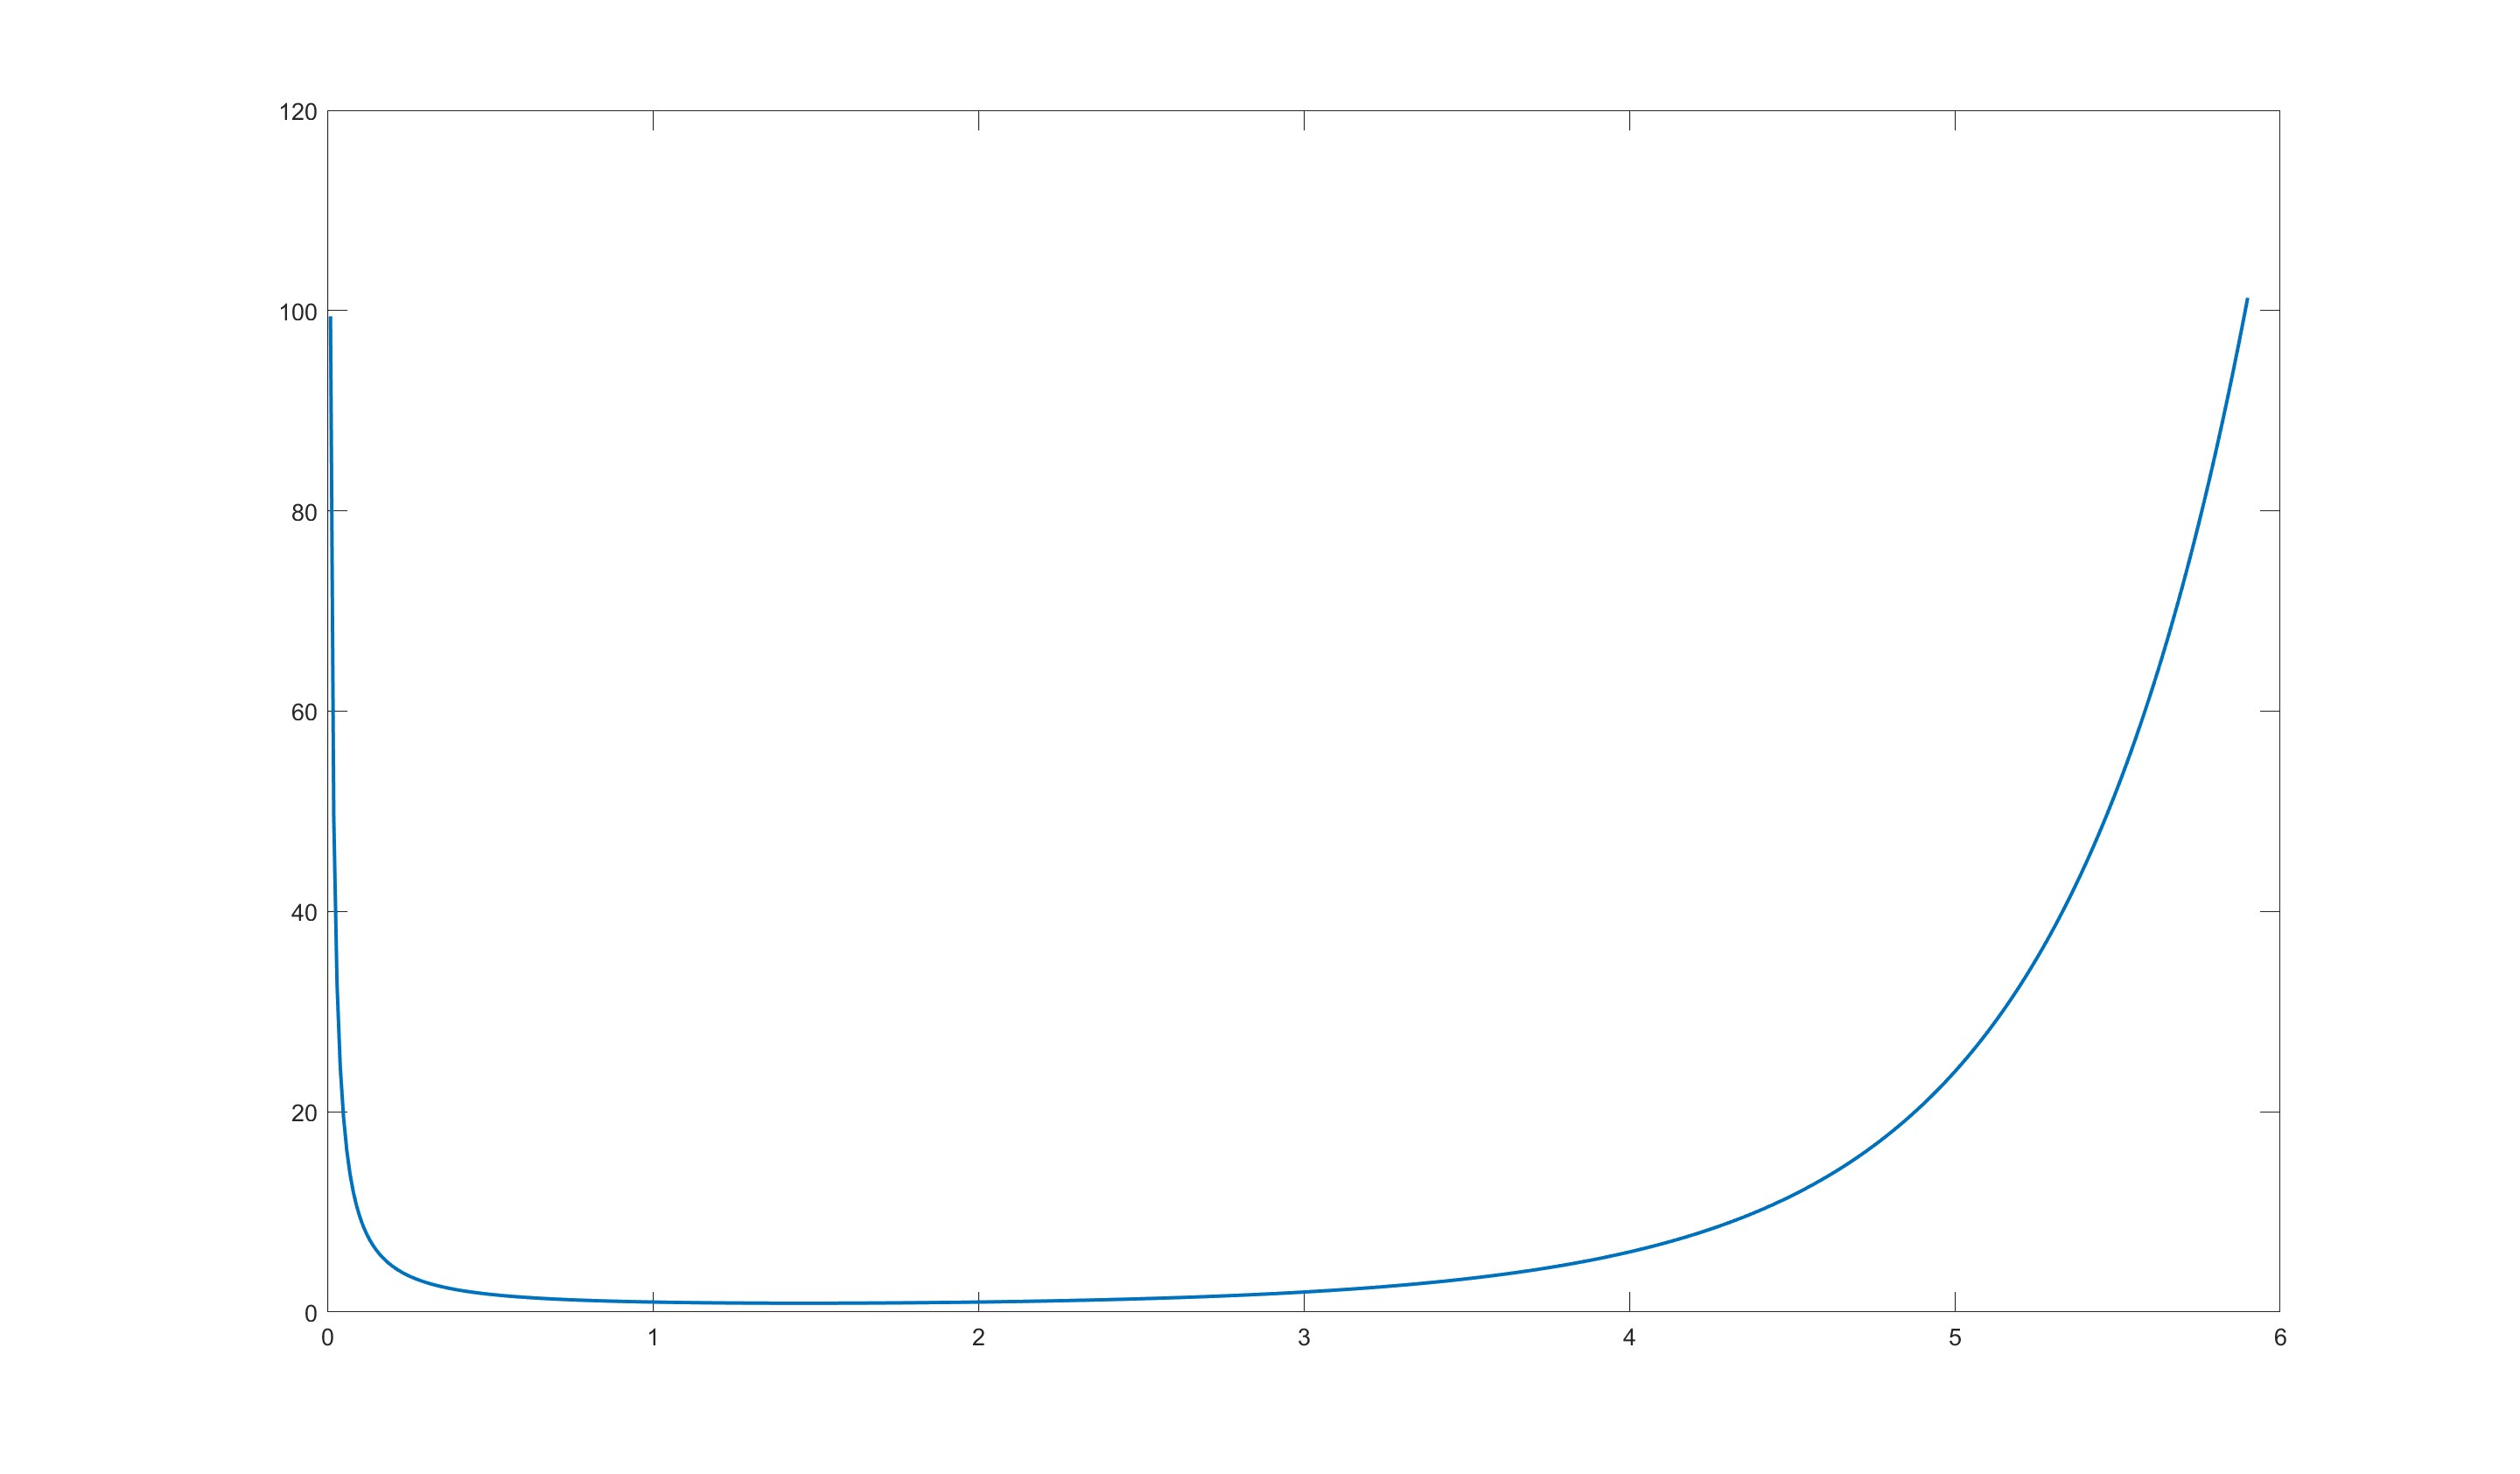
\includegraphics[width=.9\textwidth]{assets/gamma_graph.jpg}
	\caption{Grafico della funzione Gamma realizzato con MATLAB®.}
\end{figure}

La funzione è continua in $[1,2]$, e quindi per Weierstrass deve ammettere un minimo in questo intervallo. 
Poichè se esiste, a causa della monotonia della derivata il minimo deve essere anche unico, e poichè $ \Gamma(1)= \Gamma(2)$, dal Teorema di Lagrange e dal Teorema di Fermat segue che il punto di minimo della funzione è compreso tra $1$ e $2$. 
Numericamente, si trova che esso è nel punto $x_{ \min}=1,46 \dots$, con minimo $f(x_{ \min})=0,88 \dots$.

Veniamo alla relazione fondamentale del capitolo. 
\begin{Res}[Equazione funzionale della Funzione Gamma]
\label{eq_fun_gamma}
La funzione $ \Gamma: \mathbb{R} \to \mathbb{R}$ soddisfa l'equazione funzionale
	\begin{equation*}
		\Gamma(x+1)=
		x \Gamma(x).
	\end{equation*}
\end{Res}
\begin{proof}
È sufficiente integrare per parti (in modo tale da diminuire grado della potenza nell'integranda) per ricondursi alla tesi:
	\begin{equation*}
		\Gamma(x+1)= \int^{+ \infty}_0 e^{-t}t^x \: \, \mathrm{d}t =
		\int^{+ \infty}_0 x \, e^{-t}t^{x-1} \: \, \mathrm{d}t - \left[e^{-t}t^x \right]^{+ \infty}_0 =
		x \Gamma(x).
	\end{equation*}
\end{proof}
Voglio spendere due parole sull'idea, ricorrente, usata in questa dimostrazione. 
Propriamente, si usa l'identità di integrali propri
\begin{equation*}
	\int^L_0 e^{-t} t^x \: \, \mathrm{d}t = 
	\int^L_0 x \, e^{-t} t^{x-1} \: \, \mathrm{d}t - \left[e^{-t} t^x \right]^L_0,
\end{equation*}
valutata al limite. 
Questa, presenta due termini: uno che si stabilizza al crescere di $L$, e l'altro si annulla. 
In altri termini, man mano che l'intervallo su cui consideriamo l'integrale si "globalizza", il termine di bordo decade \footnote{Gli audaci che dovessero usare il Griffith per Fisica 2, riconosceranno l'uso di questa tecnica.}.

Tornando a noi, un'applicazione immediata dell'Equazione Funzionale è che possiamo valutare la velocità di divergenza.
In $x=0$,
\begin{equation*}
	\Gamma(x)= \frac{ \Gamma(x+1)}{x} \sim \frac{1}{x}
\end{equation*}
Pertanto, $ \Gamma$ diverge come la funzione $ \frac{1}{x}$ in quell'intorno. 

Valutare l'asintotico all'infinito è più difficile. 
Per farlo, partiamo da una valutazione della funzione su una classe di punti.

\begin{Res}[Valutazione di $\Gamma$ sui naturali] 
La funzione reale $ \Gamma(x)$ interpola la funzione fattoriale che ha per dominio $ \mathbb{N}$. 
In altri termini,
	\begin{equation*}
		\Gamma(n+1)=n! \quad \forall n \in \mathbb{N}.
	\end{equation*}
\end{Res}
\begin{proof}
Immediato per induzione, con caso base $ \Gamma(1)=1$.
\end{proof}
Anche se provato solo successivamente, possiamo fare ipotesi sulla velocità di crescita di $ \Gamma$: non soprenderà nessuno che valga proprio l'asintotico $ \Gamma(x) \sim x^x e^{-x} \sqrt{2 \pi x}$.


Anche altre valutazioni analitiche sono possibili grazie a questo strumento. 
Osservando che in $x= \frac{1}{2}$, attraverso la sostituzione $y^2=t$, ci si riconduce immediatamente all'integrale di Gauss, otteniamo 
\begin{equation*}
	\Gamma \left( \frac{1}{2} \right)= \int_{0}^{+ \infty}e^{-t}t^{- \frac{1}{2}} \, \mathrm{d}t=2 \int_{0}^{+ \infty}e^{-y^2} \, \mathrm{d}y= \sqrt{ \pi}.
\end{equation*} 
Utilizzando la relazione funzionale possiamo valutare $ \Gamma$ per altri valori.
\begin{Lem}[Valutazione di $\Gamma$ sui numeri della forma $n+ \frac{1}{2}$] Per $n \in \mathbb{N}$,
	\begin{equation*}
		\Gamma \left(n+ \frac{1}{2} \right) = 
		\sqrt{ \pi} \frac{(2n)!}{4^n n!}.
	\end{equation*}
\end{Lem}

Solo il seguente risultato, il teorema di Bohr-Mollerup, sottolinea però la vera forza di questa relazione. 
L'unico prerequisito per comprenderne l'enunciato è la nozione di $ \log$-convessità: si tratta di una condizione di regolarità più forte della convessità, per cui anche il logaritmo della funzione è convesso. 
Un esercizio è dimostrare che questa condizione implica la convessità. 
Senza dimostrazione \footnote{Rudin, Principles of Mathematical Analysis, Teorema 8.18.}, affermiamo che la funzione Gamma è $ \log$-convessa.

\begin{The}[Bohr-Mollerup]
Sia $f:(0,+ \infty) \to(0,+ \infty)$ tale che
\begin{enumerate}
	\item $f(1)=1$,
	\item $f(x+1)=xf(x)$ per ogni $x \in (0,+ \infty)$,
	\item $f$ è $ \log$-convessa.
\end{enumerate}
Allora, la funzione è data da
\begin{equation*}
f(x) = 
\lim_{n \to \infty} \frac{n^x n!}{x(x+1) \dots(x+n)},	
\end{equation*}
e in particolare è unica.
\end{The}
Quindi, la funzione $ \Gamma$, $ \log$-convessa che soddisfa (2), è anche l'unica con queste proprietà. 
Il teorema fornisce inoltre una caratterizzazione \footnote{Termine da matematico per "maniera di indicare un oggetto senza ambiguità, e cioè unicamente, descrivendolo attraverso delle proprietà diverse da quelle con cui è stato definito". 
Comunemente usato in Probabilità, Teoria della Misura e Geometria.} alternativa, come limite
\begin{equation*}
	\Gamma(x) = 
	\lim_{n \to \infty} \frac{n^x n!}{x(x+1) \dots(x+n)}.	
\end{equation*}

\pagebreak
% costante_eulero_mascheroni.tex
%! TeX root = ../lezione_turbo.tex
\chapter{Costante di Eulero-Mascheroni}
Durante il corso è stato dimostrato che la serie armonica $s_n= \sum^n_1 \frac{1}{k}$ è asintotica a $ \log(n)$.

In questa sezione si ricaverà che la loro differenza converge.

\begin{Res} 
	Esiste un reale $ \gamma \in \left( \frac{1}{2},1 \right)$ tale che
	\begin{equation*}
		\lim \limits_{n \to+ \infty}s_n- \log(n)= 
		\gamma.
	\end{equation*}
\end{Res}
\begin{proof}
	Il nostro piano è $s_n - \log(n)$ come un integrale, applicare la gamma di strumenti noti, e poi prendere il limite.

	Partiamo da $s_n$. 
	Vogliamo trovare una funzione $F_n$ derivabile e parametrizzata su $n$ tale che $F_n(1)=s_n$ e $F_n(0)=0$. 
	Poi, vogliamo sfruttare questa proprietà per applicare il TFC\footnote{Teorema Fondamentale del Calcolo}, per tradurre la differenza $F_n(1)-F_n(0)$ in un integrale calcolato su un intervallo fisso.
	Consideriamo il polinomio (calato dall'alto\dots)
	\begin{equation*}
		F_n : x \in [0,1] \to
		\sum^n_1 \frac{x^k}{k} \in \mathbb{R},
	\end{equation*}
	che è derivabile e rispetta i vintoli.
	L'integranda sarà la derivata di $F_n$, data da
	\begin{equation}
		\label{res1}
		f_n(x)= 
		\sum^{n-1}_0x^k= 
		\frac{x^n-1}{x-1}.
	\end{equation}	
	Osservando allora che $f$ è continua (quindi integrabile), ricaviamo
	\begin{equation*}
		s_n=
		F(1)-F(0)= 
		\int^1_0f(x) \: \mathrm{d}x= 
		\int^1_0 \frac{1-x^n}{1-x} \: \mathrm{d}x= 
		\int^1_0 \frac{1-(1-y)^n}{y} \: \mathrm{d}x,
	\end{equation*}	
	dove abbiamo applicato il TFC sulla primitiva (per costruzione) $F_n$ di $f_n$, e sostituito $y=1-x$. 
	
	Ora stiamo lavorando nel continuo. Per semplicare l'espressione (idealmente, facendo apparire un $\log n$), applichiamo l'idea spiegata nel commento al Risultato \ref{eq_fun_gamma}: spezziamo l'integrale in due, e mostriamo che uno dei due contributi decade.
	In particolare, definiamo
	\begin{gather*}
		s_n = 
		\mathcal{I}_n + \mathcal{J}_n \quad \text{dove} \\
		\mathcal{I}_n = \int^1_0 \frac{1-e^{-nx}}{x} \: \mathrm{d} x 
		\qquad 
		\mathcal{J}_n= \int^1_0 \frac{e^{-nx}-(1-x)^n}{x} \: \mathrm{d} x.
	\end{gather*}
	
	\begin{figure}
		\centering
		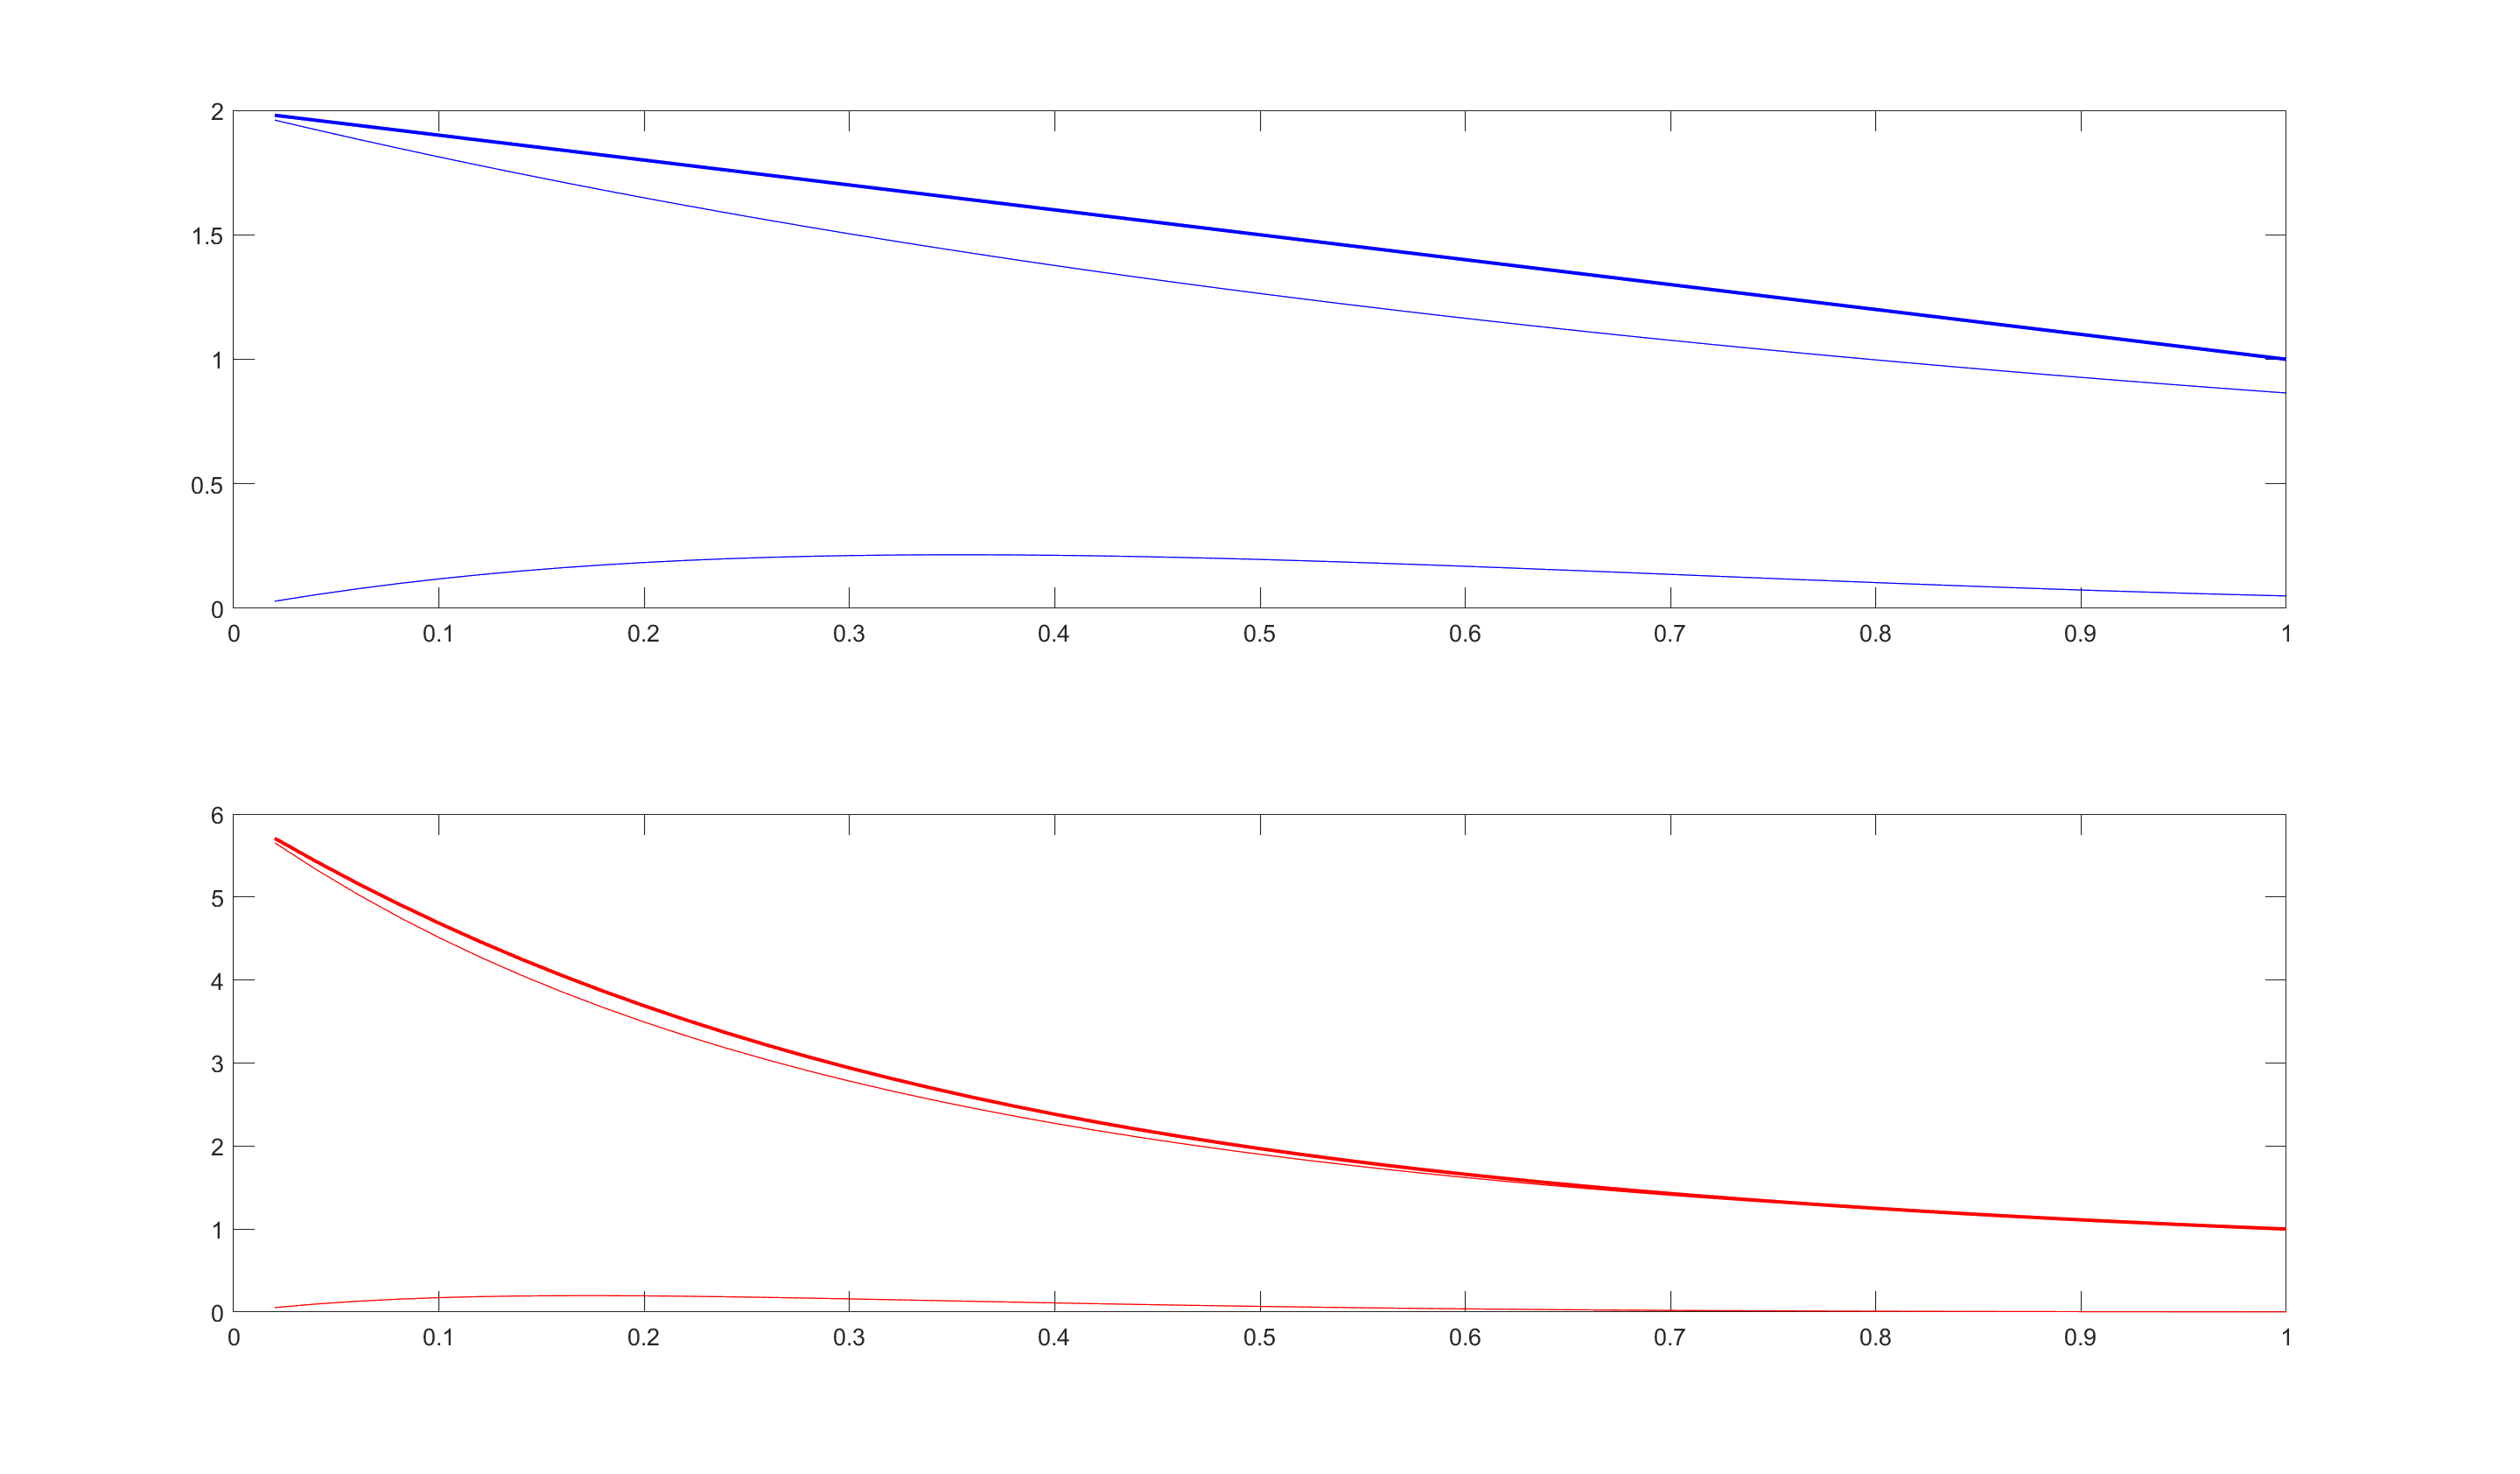
\includegraphics[width=.9\textwidth]{assets/eulero_mascheroni_choice.png}
		\caption{Le tre funzioni integrande ($f_n$ in grassetto), per $n=3$ e per $n=6$}.		
	\end{figure}

	Dalla figura, è chiaro che $\mathcal{J}_n$ decada. 
	A riprova di ciò, se uno considera il limite $f_n(x)$ per ogni $x \in \left( 0,1 \right]$, calcolato espandendo il polinomio di Taylor, trova che si annulla. Per $x=0$ la funzione non è definita, ma può essere estesa con continuità per ogni $n$, secondo il limite
	\begin{equation*}
		\lim \limits_{x \to0} \frac{e^{-nx}-(1-x)^n}{x}= 
		\lim \limits_{x \to0} \frac{o(x)}{x}=
		0,
	\end{equation*}
	calcolato di nuovo sviluppando l'esponenziale con Taylor.

	Questa è un'applicazione immediata del teorema di Convergenza Dominata, ma nello spirito di questa lezione è stato deciso di fare una dimostazione solo di AM1.

	
	
	% Allora, per dei risultati sulle successioni funzionali (in particolare, la convergenza uniforme $f_n \rightrightarrows f$ e continuità di $f_n$), si ottiene che
	% \begin{equation*}
	% 	\lim \limits_{n \to+ \infty} \int^1_0f_n(x) \: \mathrm{d}x= 
	% 	\int^1_0 \lim \limits_{n \to+ \infty}f_n(x) \: \mathrm{d}x=
	% 	\int^1_00 \: \mathrm{d}x=
	% 	0.
	% \end{equation*}

	% In conclusione $ \lim \limits_{n \to+ \infty} \mathcal{J}_n=0$ e si può dimostrare che $ \mathcal{J}_n \sim \frac{1}{2n}$.

	Ora analizziamo $ \mathcal{I}_n$. 
	L'integrale è improprio, e presenterebbe un punto critico in $x=0$. 
	In realtà, l'integranda converge per le gerarchie d'infinito e quindi è integrabile secondo Riemann su tutto l'intervallo.

	L'integrale può essere semplificato fino a raggiungere la forma "$ \log x +f(x)$": si sostituisca $t=nx$ e poi si integri per parti.
	\begin{align*}
			\mathcal{I}_n= 
			\int^1_0 \frac{1-e^{-nx}}{x} \: \mathrm{d}x
			&= 
			\int^n_0 \frac{1-e^{-t}}{t} \: \mathrm{d}t= 
			\\ &= 
			\left[ \left(1-e^{-t} \right) \log t \right]^n_0 - \int^n_0 e^{-t} \log t \: \mathrm{d}t=
			\\ &=
			\log n-e^{-n} \log n- \int^n_0e^{-t} \log t \: \mathrm{d}t.
	\end{align*}

	Sostituendo la precedente identità nella differenza tra $s_n$ e $ \log n$ otteniamo
	\begin{equation*}
		s_n- \log n= 
		\mathcal{J}_n+ \mathcal{I}_n- \log n= 
		\mathcal{J}_n-e^{-n} \log n- \int^n_0 e^{-t} \log t \: \mathrm{d}t.
	\end{equation*}

	Poichè $ \lim_{n \to \infty} \mathcal{J}_n=0$ e $ \lim_{n \to \infty} e^{-n} \log n=0$, si ricava una formula che permette di trovare la costante con precisione arbitraria:
	\begin{equation*}
		\gamma= 
		\lim \limits_{n \to+ \infty}(s_n- \log n)=
		- \int^{+ \infty}_0e^{-t} \log t \: \mathrm{d}t.
	\end{equation*}

	Un'osservazione interessante, infine, è che questo integrale può essere ricondotto alla Funzione Gamma.	
	Infatti, la derivata $ \Gamma'(x)$, calcolata applicando il Teorema di Lebesegue (e cioè invertendo l'ordine di derivazione e integrazione), soddisfa la relazione
	\begin{align*}
		\Gamma'(x)&= 
		\frac{ \mathrm{d}}{ \mathrm{d}x} \left( \int^{+ \infty}_0e^{-t} \: t^{ \,x-1} \mathrm{d}t \right) = 
		\\ &= 
		\int^{+ \infty}_0 \frac{ \mathrm{d}}{ \mathrm{d}x} \left( e^{-t} \: t^{ \,x-1} \right) \mathrm{d}t= 
		\\ &= 
		\int^{+ \infty}_0e^{-t} \: t^{ \,x-1} \log t \: \mathrm{d}t
	\end{align*}
	Da cui si deduce che $ \gamma=- \Gamma'(1)$, che numericamente equivale a $0,577 \dots$
\end{proof}
\pagebreak
% approx_de_moivre_sterling.tex
%! TeX root = ../lezione_turbo.tex
\chapter{Formula di De Moivre-Sterling}
Durante il Corso è stata impiegato spesso l'asintotico tra il fattoriale e la formula di De Moivre-Stirling. Questa fornisce una dimostrazione formale della relazione.

\begin{Res} Vale l'uguaglianza asintotica
	\[
		n!\sim n^ne^{-n}\sqrt{2n\pi}.
	\]
\end{Res}

\begin{proof}
	Dimostreremo che
	\[
		n! = n^n e^{-n} \sqrt{n} \, p_n	
	\]
	dove $p_n\to\sqrt{2\pi}$ per $n \to \infty$. Per farlo, impiegheremo gli strumenti analitici del continuo al posto di quelli della matematica discreta, in modo tale da produrre funzioni come gli esponenziali della formula. Poichè la funzione fattoriale non ha un'estensione reale banale, ne usiamo una interpolazione sui reali. Alla luce dei risultati precedenti, è naturale impiegare la funzione Gamma. Essa è molto regolare$(C^\infty
	%$ e $\Gamma \leq 0
	)$, e quindi si presta a manipolazioni analitiche. Ricordiamo infatti che vale
	\[
		n!=\Gamma(n+1)=\int^{+\infty}_0e^{-t}t^n \:\mathrm{d}t,
	\]
	per ogni intero positivo $n$.

	L'approccio dimostrativo diventa quello di estrarre dall'integrale di destra gli elementi della formula di De Moivre-Sterling.

	Sostituiamo $t=n(u+1)$:
	\[
		n!=n^ne^{-n}\int^{+\infty}_{-1}n\left( e^{-u}(1+u)\right)^n \:\mathrm{d}u.
	\]
	A questo punto, eliminiamo il fattore moltiplicativo $1+u$ incorporandolo nell'esponenziale. Definiamo cioè una funzione continua $h(u)$ che soddisfi

	\begin{equation}
		\label{res2}
		e^{-u}(1+u)=e^{-u^2 h(u)} \implies -u+\log(1+u)=-u^2h(u).
	\end{equation}

	Risolvendo l'equazione ed estendendo $h$ con continuità in $x=0$, otteniamo che
	\begin{equation*}
		h(u)=
		\begin{cases}
			(u-log(1+u))\frac{1}{u^2} & \text{se } u\neq0, \\
			\frac{1}{2}               & \text{se }  u=0.
		\end{cases}
	\end{equation*}

	Sostituendo questa funzione nell'integrale ed effettuando il cambio di variabile $t=u\sqrt{n}$ si ottiene l'identità
	\begin{equation*}
		n^ne^{-n}\int^{+\infty}_{-1}n\left( e^{-u}(1+u)\right)^n \:\mathrm{d}u=
		n^ne^{-n}\sqrt{n}\int^{+\infty}_{-\sqrt{n}} e^{-t^2h\left(\frac{t}{\sqrt{n}}\right)} \:\mathrm{d}t.
	\end{equation*}
	Rimane quindi da verificare che
	\[
		p_n = \int^{+\infty}_{-\sqrt{n}} e^{-t^2h\left(\frac{t}{\sqrt{n}}\right)} \:\mathrm{d}t = \int^{+\infty}_{-\infty} e^{-t^2h\left(\frac{t}{\sqrt{n}}\right)} \chi_n(t) \:\mathrm{d}t,
	\]
	dove $\chi_n(x)$ indica la funzione indicatrice di $\left[-\sqrt{n},+\infty\right]$ valutata in $x$, converge a $\sqrt{2\pi}$.

	Si definisca $f_n(t)= e^{-t^2h\left(\frac{t}{\sqrt{n}}\right)}\chi_n(t)$. Grazie alla continuità di $h(c)$ e della funzione esponenziale risulta che $\lim f_n(t)=e^{-\frac{1}{2}t^2}$ per ogni $t$\footnote{In Analisi 2, si dirà che la successione di funzioni $f_n$ tende alla funzione $e^{-\frac{1}{2}t^2}$ \textit{puntualmente}, un tipo di convergenza funzionale debole.}.

	\goodbreak Per il teorema della Convergenza Dominata di Lebesgue\footnote{Si tratta di un risultato di Teoria della Misura sulle successioni di funzioni. Verrà affrotato in Probabilità e Analisi 3.}, commutiamo l'integrazione e il limite\footnote{Esplicitamente, si valuta prima l'integranda al limite e poi si integra il risultato.}.
	\goodbreak\begin{multline}
		\lim\limits_{n\to+\infty} p_n = \lim\limits_{n\to+\infty}\int^{+\infty}_{-\infty} e^{-t^2h\left(\frac{t}{\sqrt{n}}\right)} \chi_n(t) \:\mathrm{d}t=\\
		=\int^{+\infty}_{-\infty}e^{-\frac{1}{2}t^2}\:\mathrm{d}t=\sqrt{2}\int^{+\infty}_{-\infty}e^{-u^2}\:\mathrm{d}u=\sqrt{2\pi},		
	\end{multline}
	dove abbiamo sostituito $u^2=\frac{t^2}{2}$ per ricavare la costante $\sqrt{2}$, e abbiamo sostituito l'integrale di Gauss.
\end{proof}
Questa dimostrazione fornisce anche un asintotico reale per $\Gamma(x)$, oltre che un asintotico discret per $n!$.
\pagebreak
% sophomore_dream.tex
%! TeX root = ../lezione_turbo.tex
\chapter{Sophomore's Dream}
Il risultato di Bernoulli che in assoluto suscitò più clamore nella comunità matematica del tempo fu un'identità che passò alla storia con il nome Sophomore's Dream, in contrapposizione con la falsa uguaglianza
\begin{equation*}
	(x+y)^n=
	x^n+y^n,
\end{equation*}
nota come Freshman's Dream.
\begin{Res}[Sophomore's Dream]
	\begin{equation}
		\int^1_0x^{-x} \: \mathrm{d}x= 
		\sum^{+ \infty}_1n^{-n}
	\end{equation}
\end{Res}
La dimostrazione dell'identità si basa su un lemma che Bernoulli provò integrando induttivamente per parti su $k$, ma che noi dimostreremo in maniera più elegante usando i risultati visti finora.
\begin{Lem}
	\label{lemma_sophomore}
Per ogni coppia di valori naturali $n$ e $k$ si verifica che
	\begin{equation*}
		\int^1_0x^n( \log(x))^k \: \mathrm{d}x=
		(-1)^k \frac{k!}{(n+1)^{k+1}}
	\end{equation*}
\end{Lem}
\begin{proof}[Dimostrazione - Lemma]
	Seguendo un approccio diverso a quello del capitolo precedente, impieghiamo la funzione Gamma come estensione reale del fattoriale e applichiamo gli strumenti analitici del continuo. 
	Sostituiamo $x=e^{-t}$ e utilizziamo la proprietà dell'integrale definito:
	\begin{equation*}
		\begin{split}
			\int^1_0x^n( \log(x))^k \: \mathrm{d}x
			&= 
			\int_{+ \infty}^0e^{-tn} \left( \log \left(e^{-t} \right) \right)^k \left(-e^{-t} \right) \: \mathrm{d}t= 
			\\ &=
			(-1)^k \int^{+ \infty}_0e^{-(n+1)t} \, t^k \: \mathrm{d}t.
		\end{split}
	\end{equation*}
	E per concludere sostituiamo $(n+1)t=y$:
	\begin{equation*}
		(-1)^k \int^{+ \infty}_0e^{-y} \, \frac{y^k}{(n+1)^{k+1}} \: \mathrm{d}y= 
		\frac{(-1)^k}{(n+1)^{k+1}} \int^{+ \infty}_0e^{-y}y^k \: \mathrm{d}y.
	\end{equation*}
	Infine, osserviamo che l'integrale del termine di destra è pari a $ \Gamma(k+1)=k!$, da cui segue la tesi.
\end{proof}
\begin{proof}[Dimostrazione - Sophomore's Dream]
	Richiamiamo che $e^q= \sum^{+ \infty}_0 \frac{q^n}{n!}$, e sostituendo $q$ otteniamo
	\begin{equation*}
		x^{-x}=e^{-x \log(x)}= 
		\sum^{+ \infty}_0 \frac{(-x \log(x))^n}{n!}.
	\end{equation*}
	E quindi vale l'identità
	\begin{equation*}
		\int^1_0x^{-x} \: \mathrm{d}x= 
		\int^1_0 \sum^{+ \infty}_0 \frac{(-x \log(x))^n}{n!} \: \mathrm{d}x,
	\end{equation*}
	dove, applicando dei risultati sulle successioni di funzioni (in particolare, l'uniforme continuità e l'integrabilità delle funzioni), possiamo invertire l'integrale e la sommatoria, ricavando
	\begin{equation*}
		\int^1_0 \sum^{+ \infty}_0 \frac{(-x \log(x))^n}{n!} \: \mathrm{d}x= 
		\sum^{+ \infty}_0 \frac{(-1)^n}{n!} \int^1_0(x \log(x))^n \: \mathrm{d}x.
	\end{equation*}
	Applicando il Lemma \ref{lemma_sophomore} e semplificando, otteniamo la tesi.
	\begin{equation*}
		\int^1_0x^{-x} \: \mathrm{d}x= 
		\sum^{+ \infty}_0 \frac{1}{(n+1)^{n+1}}= 
		\sum^{+ \infty}_1n^{-n}.
	\end{equation*}
\end{proof}
Il lemma che abbiamo dimostrato è piuttosto potente e può essere impiegato per trovare anche altri integrali.
\begin{Res} 
	Calcolare
	\begin{equation*}
		\int^1_0 \frac{ \log(x)}{x-1} \: \mathrm{d}x
	\end{equation*}
\end{Res}
\begin{proof}[Calcolo]
	L'integrale è improprio. 
	I punti critici sono $0$ ed $1$: nell'intorno di $0$ l'integranda è asintotica a $ \log(x)$, e nell'intorno di $1$ il numeratore è asintotico ad $x-1$, entrambe funzioni integrabili. 
	Quindi, per il criterio asintotico la funzione è integrabile.

	Questo integrale non ammette una primitiva in termini di funzioni elementari: per calcolarlo, lo riformuliamo in termini del Lemma \ref{lemma_sophomore}. 
	Osserviamo che
	\begin{equation*}
		\int^1_0 \frac{ \log(x)}{x-1} \: \mathrm{d}x=
		- \int^1_0 \log(x) \, \frac{1}{1-x} \: \mathrm{d}x=
		- \int^1_0 \log(x) \, \sum^{+ \infty}_0(x^n) \: \mathrm{d}x,
	\end{equation*}
	dove nell'ultimo passaggio abbiamo sostituito la somma della serie geometrica $ \frac{1}{1-x}$, sfruttando il fatto che $x$ è compreso tra $0$ ed $1$.

	Applicando nuovamente dei risultati sulle successioni di funzioni,
	\begin{equation*}
	- \int^1_0 \left( \log(x) \right) \sum^{+ \infty}_0(x^n) \: \mathrm{d}x=
	- \sum^{+ \infty}_0 \int^1_0x^n \log(x) \: \mathrm{d}x.
	\end{equation*}
	Ora è sufficiente sostituire il lemma e svolgere delle semplificazioni per ottenere che
	\begin{equation*}
	- \sum^{+ \infty}_0 \int^1_0x^n \log(x) \: \mathrm{d}x=
	\sum^{+ \infty}_{0} \frac{1}{(n+1)^2}= 
	\sum^{+ \infty}_{1}n^{-2}= 
	\frac{ \pi^2}{6}.
	\end{equation*}
\end{proof}
Curiosamente, questo integrale si può calcolare anche invertendo il numeratore e il denominatore.
\begin{Res} Calcolare
	\begin{equation*}
		\int^1_0 \frac{x-1}{ \log(x)} \: \mathrm{d}x
	\end{equation*}
\end{Res}
\begin{proof}[Calcolo]
	In primo luogo, dimostriamo l'integrabilità impropria in maniera analoga al risulato precedente.

	La tecnica necessaria per calcolare questo integrale è quella dell'integrale di Faymann. 
	In pratica, si definisce una funzione che generalizzi l'integrale e, attraverso la derivazione, si trova il valore che ci interessa come caso particolare del risultato generale. 
	Operativamente, si definisce
	\begin{equation*}
		\mathrm{F}(t)= 
		\int^1_0 \frac{x^t-1}{ \log(x)} \: \mathrm{d}x
	\end{equation*}
	e si determina $ \mathrm{F}(1)$. 
	Per farlo, applicheremo Lagrange. 
	Osserviamo che $ \mathrm{F}(0)=0$, e deriviamo la funzione $ \mathrm{F}$. 
	Postulando che siano verificate le ipotesi necessarie, deriviamo integriamo la derivata dell'integranda rispetto a $t$, e cioè
	\begin{equation*}
		\mathrm{F}'(t)= 
		\int^1_0 \left( \frac{x^t-1}{ \log(x)} \right)' \: \mathrm{d}x= 
		\int^1_0x^t \: \mathrm{d}t= 
		\frac{1}{1+t}.
	\end{equation*}
	Da cui, per Lagrange,
	\begin{equation*}
		\mathrm{F}(t)= 
		\mathrm{F}(t)- \mathrm{F}(0)= 
		\int^1_0x^t \: \mathrm{d}t= 
		\int^1_0 \frac{1}{1+t} \: \mathrm{d}x= 
		\left[ \log(1+t) \right]^1_0.
	\end{equation*}
	Valutando l'ultimo termine otteniamo che l'integrale di partenza vale $ \log(2)$.
\end{proof}

\end{document}